\documentclass[12pt,a4paper]{article}
\usepackage{fontspec}
\setmainfont{PT Serif}
\usepackage{polyglossia}
\setdefaultlanguage{russian}
\newfontfamily\cyrillicfont{PT Serif}
\newfontfamily\cyrillicfontsf{PT Sans}
\newfontfamily\cyrillicfonttt{PT Mono}
\newfontfamily\transcriptfont{Arial Unicode MS}
\usepackage[a4paper,margin=22mm]{geometry}
\usepackage{microtype}
\usepackage{graphicx}
\usepackage{array,tabularx,longtable,multirow,makecell}
\usepackage{pdflscape}
\usepackage{pdfpages}
\usepackage{fancyvrb}
\usepackage{fvextra}
\usepackage{tikz}
\usetikzlibrary{arrows.meta,positioning,calc,patterns,shapes.geometric,shapes.misc}
\usepackage{caption}
\captionsetup[figure]{labelformat=empty}
\usepackage{hyperref}
\hypersetup{colorlinks=true,linkcolor=black,urlcolor=blue,citecolor=black}
\setlength{\parindent}{1.1em}
\setlength{\parskip}{0.2em}
\renewcommand{\arraystretch}{1.15}
\newcommand{\vhead}[1]{\rotatebox[origin=c]{90}{\scriptsize #1}}
\newcommand{\vheadland}[1]{\rotatebox[origin=c]{90}{\parbox{2.8cm}{\centering\scriptsize #1}}}
\newcolumntype{V}{>{\centering\arraybackslash}p{1.2cm}}
\newcommand{\blankrow}{\rule{0pt}{0.55cm}}
\newcommand{\sourcepage}[1]{\textit{Источник: том 5, с. #1.}}
\newcommand{\formsource}[2]{\par\noindent{\footnotesize\textit{Источник: S-02, с. #1; S-01, с. #2.}}\par\vspace{0.2em}}
\newcommand{\formmetadata}[1]{\par\noindent\begin{minipage}[t]{\linewidth}\raggedright #1\end{minipage}\par\smallskip}

\title{Система «СПУТНИК» и технические средства отображения в системе «СКАЛАР-2»\\[0.5em]
\large Источниковое воспроизведение методики и первичных материалов}
\author{Редакционная компиляция проекта\\
\small Авторы основного текста книги 1996 года:\\
Р. И. Образцова, П. Г. Кузнецов,\\
С. Б. Пшеничников}
\date{Рабочая редакция источникового воспроизведения}

\begin{document}
\maketitle
\clearpage

\begin{quote}\small
\textbf{О границах этой редакции.} Здесь воспроизведены разделы 6.3--6.4 книги 1996 года (печатные страницы 111--118), приложение 2 «Система СПУТНИК» (страницы 173--187 книги 1996 года; перепечатка в томе 5, страницы 111--125) и приложение 3 о технических средствах СКАЛАР-2 (страницы 187--189 книги 1996 года; том 5, страницы 126--129). Дополнительные первичные тексты тома 5, страницы 11--110, даны отдельной поисковой транскрипцией; полные факсимиле страниц 11--129 тома 5 и страниц 111--118 книги 1996 года приложены в конце. Разделы 6.3--6.4 в томе 5 не перепечатаны; это самостоятельная часть основного текста книги. Редакторские сноски тома 5 указывают источник приложений. Рисунки П.3 и П.4 в томе 5 перенесены с рисунков 13 и 14 книги 1996 года, страницы 114.

Таблица П.9 сохраняет шесть вопросов источника: «Кто, Что, Когда, Где, Сколько, Как». В ней нет вопроса «Почему» и нет термина 5W2H. Их сопоставление в проектных материалах — аналитическая рамка исследования, не часть воспроизводимого авторского текста.

В корпусе сохранены два исходных PDF без изменений. Реестр первичных материалов описывает авторство и редакционные границы всех текстов тома 5, вошедших в поисковую выгрузку. Выгрузка страниц 11--110 не вычитана по изображениям и нужна для поиска; её ошибки не являются авторскими формулировками.

Постраничные тексты получены из текстовых слоёв двух PDF и сохраняют разбиение по страницам. Для S-01, страницы 111--118, текст визуально сверялся со сканами; исходная выгрузка сохранена отдельно. В секции S-02, страницы 111--129, повреждённые OCR-таблицы исключены из сплошной транскрипции, а формы П.1--П.9 набраны ниже по изображениям источника; исходная выгрузка сохранена в `sources/transcriptions`. Транскрипция S-02 и дополнительный текстовый слой страниц 11--110 могут содержать ошибки распознавания; используйте оригиналы как контрольные страницы. Рисунок П.4 дан в векторной трассировке по скану S-02, с. 129; рядом сохранено точное факсимиле рисунка для контроля.

У книги 1996 года есть явное уведомление об авторском праве. Для тома 5 в проверенных выходных данных открытая лицензия не указана. Эта редакция сохраняет авторство и не заявляет свободной лицензии на источники.
\end{quote}

\clearpage
\tableofcontents

\section{Основной текст книги 1996 года: СКАЛАР и сетевые модели}

Разделы 6.3--6.4 S-01 (печатные страницы 111--118) содержат описание строки плана СКАЛАР, шести типов управленческих решений и перехода к сетевой модели СПУТНИК. Этот текст не входит в перепечатанные приложения. Транскрипция ниже сверена постранично с изображениями S-01; исходная выгрузка текстового слоя сохранена в каталоге источников. Рисунки 13--14 с печатной страницы 114 воспроизведены позднее в томе 5 как рисунки П.3--П.4.

\begingroup
\footnotesize
\VerbatimInput[fontsize=\footnotesize,breaklines=true,breakanywhere=true]{source-transcription-book-1996-111-118.txt}
\endgroup

\subsection{Стандартная строка плана СКАЛАР}

Печатная страница 113 задаёт порядок граф следующим образом. Геометрия таблицы набрана заново; факсимиле страницы 113 остаётся доступным в S-01.

\footnotesize
\setlength{\tabcolsep}{2pt}
\begin{tabularx}{\linewidth}{|c|p{1.6cm}|c|X|X|X|X|X|X|}\hline
№ п/п&Кодовый номер&Кто&Что&Когда&Где&Сколько&Как&Замечание\\\hline
&&&&&&&&\\\hline
&&&&&&&&\\\hline
&&&&&&&&\\\hline
\end{tabularx}

\section{Постраничная транскрипция источника}

Дополнительные самостоятельные тексты тома 5 (печатные страницы 11--110) включают отчёт об опыте СПУ, два ранних текста о СПУТНИК, статью «Системы СПУТНИК», текст о СПУТНИК-СКАЛАР, введение к СКАЛАР-2 и работу о системно-морфологическом планировании. Их авторство и страницы перечислены в реестре. Ниже дана необработанная поисковая выгрузка; она содержит ошибки распознавания и редакционные примечания, поэтому не заменяет чтение соответствующих страниц оригинала.

\begingroup
\footnotesize
\VerbatimInput[fontsize=\footnotesize,breaklines=true,breakanywhere=true,formatcom=\transcriptfont]{../sources/transcriptions/Vol5-2021-primary-pages-11-110-raw.txt}
\endgroup

\section{Постраничная транскрипция приложений СПУТНИК / СКАЛАР-2}

Текстовый слой S-02, страницы 111--129, воспроизведён постранично. Он содержит текст процедур СПУТНИК, техническое описание СКАЛАР-2 и подписи рисунков. OCR-выгрузка табличных полей сохранена отдельно, но не печатается здесь из-за перевёрнутых и нечитаемых заголовков. Формы П.1--П.9 восстановлены по изображениям на соответствующих страницах и снабжены ссылками на страницы S-02 и S-01.

\begingroup
\footnotesize
\VerbatimInput[fontsize=\footnotesize,breaklines=true,breakanywhere=true]{source-transcription-vol5-111-129.txt}
\endgroup

\section{Векторные перерисовки схем}

\subsection{Рисунок П.1. Блок-схема развертывания работ по новой теме}

Нумерация процедур, названия документов и два класса потоков сохранены по источнику. Линии расположены заново ради читаемости. Сплошная стрелка показывает обязательный поток информации; пунктирная — возможный поток; петля со звездочкой отмечает повтор процедуры по тематическому заданию. В оригинале рисунок занимает две страницы.

\begin{figure}[p]
\centering
\begin{tikzpicture}[
  font=\scriptsize,
  proc/.style={draw,rounded rectangle,align=center,text width=8.0cm,minimum height=1.4cm,inner sep=4pt},
  doc/.style={draw,rectangle,align=center,text width=2.9cm,minimum height=0.72cm,inner sep=2pt},
  flow/.style={-{Latex[length=2mm]},thick},
  maybe/.style={-{Latex[length=2mm]},thick,dashed},
  every node/.style={outer sep=1pt}
]
\node[font=\bfseries,text width=4.8cm,align=center] at (-5.9,1.65) {Рассогласование};
\node[font=\bfseries,text width=8.0cm,align=center] at (1.3,1.65) {Нормальное развертывание работ по теме};
\draw[dashed,thick] (-3.3,0.9) -- (-3.3,-19.8);
\node[doc,text width=4.8cm] (tz) at (1.3,0) {Техническое задание (ТЗ) от заказчика};
\node[proc] (p1) at (1.3,-1.65) {\textbf{№ 1. Последовательная передача ответственности за выполнение заданий подчинённым}\par{\scriptsize РП$_0$}\par Назначение ЦР$_0$, передача ТЗ ЦР$_0$; РП$_0$ может вернуть ТЗ заказчику};
\node[doc] (d1a) at (-0.5,-3.45) {Техническое задание (ТЗ)};
\node[doc] (d1b) at (3.1,-3.45) {Приказ о назначении ЦР$_0$};
\node[proc] (p2) at (1.3,-5.25) {\textbf{№ 2. Передача ответственности за выполнение заданий подчинённым}\par{\scriptsize ЦР$_0$ (СПЦ$_0$)}\par Последовательное разбиение заданий на подзадачи, назначение ответственных за подзадачи, регистрация заданий и связей между ответственными исполнителями};
\node[doc] (d2a) at (-0.5,-7.05) {Задание № 1};
\node[doc] (d2b) at (3.1,-7.05) {Приказ о назначении};
\node[proc] (p3) at (1.3,-8.85) {\textbf{№ 3. Выдача заданий на элементы части темы}\par{\scriptsize ЦР$_{0,1}$ (СПЦ$_{0,1}$)}\par Разбиение задачи на подзадачи до уровня ответственного исполнителя работ; регистрация и формирование ЗСД (ф. 10)};
\node[doc] (d3) at (1.3,-10.55) {Запрос на сетевую документацию (ЗСД), ф. 10};
\node[proc] (p4) at (1.3,-12.35) {\textbf{№ 4. Подготовка и выдача исходных данных работ}\par{\scriptsize ОИР}\par Составление сетевого графика работ; заполнение СЧТ (ф. 11) и ИДР (ф. 12)};
\node[doc] (d4a) at (-0.5,-14.05) {СЧТ, форма 11};
\node[doc] (d4b) at (3.1,-14.05) {ИДР, форма 12};
\node[proc] (p5) at (1.3,-15.85) {\textbf{№ 5. Получение полной сети работ по теме}\par{\scriptsize СПЦ, ЦР, ОИР}\par Сшивание сетей на разработку темы; устранение неувязок};
\node[doc] (d5) at (1.3,-17.55) {Полный сетевой график разработки темы};
\node[proc] (p7) at (1.3,-19.35) {\textbf{№ 7. Определение общей продолжительности разработки темы}\par{\scriptsize СПЦ$_0$}\par Расчёт сети, нахождение общей продолжительности разработки темы};
\node[proc,text width=4.8cm] (p6) at (-5.9,-15.85) {\textbf{№ 6. Устранение неувязок плана}\par{\scriptsize ОИР, ЦР, СПЦ}\par Согласование};
\node[doc,text width=4.5cm] (mismatch) at (-5.9,-14.05) {Неувязки сетевого графика на тему};
\node[doc,text width=4.5cm] (return) at (-5.9,-1.65) {Возврат ТЗ заказчику};
\node[font=\bfseries] at (5.7,-1.65) {*};
\node[font=\bfseries] at (5.7,-5.25) {*};
\node[font=\bfseries] at (5.7,-8.85) {*};

\draw[flow] (tz) -- (p1);
\draw[flow] (p1.south) -- ++(0,-0.3) -| (d1a.north);
\draw[flow] (p1.south) -- ++(0,-0.3) -| (d1b.north);
\draw[flow] (d1a.south) -- ++(0,-0.3) -| (p2.north);
\draw[flow] (d1b.south) -- ++(0,-0.3) -| (p2.north);
\draw[flow] (p2.south) -- ++(0,-0.3) -| (d2a.north);
\draw[flow] (p2.south) -- ++(0,-0.3) -| (d2b.north);
\draw[flow] (d2a.south) -- ++(0,-0.3) -| (p3.north);
\draw[flow] (d2b.south) -- ++(0,-0.3) -| (p3.north);
\draw[flow] (p3) -- (d3);
\draw[flow] (d3) -- (p4);
\draw[flow] (p4.south) -- ++(0,-0.3) -| (d4a.north);
\draw[flow] (p4.south) -- ++(0,-0.3) -| (d4b.north);
\draw[flow] (d4a.south) -- ++(0,-0.3) -| (p5.north);
\draw[flow] (d4b.south) -- ++(0,-0.3) -| (p5.north);
\draw[flow] (p5) -- (d5);
\draw[flow] (d5) -- (p7);
\draw[maybe] (p1.west) -| (return.east);
\foreach \y in {-5.25,-8.85,-12.35}{\draw[maybe] (-8.2,\y) -- (-2.7,\y);}
\draw[maybe] (p5.west) -- (mismatch.east);
\draw[flow] (mismatch) -- (p6);
\draw[maybe] (p6.east) |- (p5.west);
\node[align=left,font=\scriptsize] at (-5.9,-18.3) {Пунктир — возможный поток\\* — процедура повторяется};
\end{tikzpicture}
\caption{Рис. П.1. Блок-схема развёртывания работ по новой теме с использованием системы СПУТНИК-1, часть 1.\\Перерисовано по S-02, с. 113.}
\end{figure}

\begin{figure}[p]
\centering
\begin{tikzpicture}[
  font=\scriptsize,
  proc/.style={draw,rounded rectangle,align=center,text width=6.0cm,minimum height=1.35cm,inner sep=3pt},
  doc/.style={draw,rectangle,align=center,text width=2.6cm,minimum height=0.72cm,inner sep=2pt},
  flow/.style={-{Latex[length=2mm]},thick},
  maybe/.style={-{Latex[length=2mm]},thick,dashed}
]
\node[font=\bfseries,text width=6.0cm,align=center] at (0.4,1.1) {Рассмотрение плана и управление программой};
\draw[dashed,thick] (-3.5,0.55) -- (-3.5,-5.7);
\node[doc,text width=3.1cm] (mismatch) at (-5.8,0.05) {Неувязки сетевого графика на тему};
\node[doc,text width=3.1cm] (draft) at (0.4,0.05) {Проект плана-графика разработки темы};
\node[doc,text width=2.4cm] (requests) at (6.3,0.05) {Заявки в службы обеспечения};
\node[proc] (p8) at (0.4,-1.9) {\textbf{№ 8. Обсуждение проекта плана-графика разработки темы}\par{\scriptsize РП$_0$ (СПЦ$_0$)}\par Сравнение плана; утверждение или неутверждение сети разработки темы};
\node[doc,text width=2.9cm] (unacceptable) at (-5.8,-0.85) {Решение о неприемлемости проекта плана-графика};
\node[proc,text width=3.4cm,minimum height=1.55cm] (p9) at (-5.8,-2.9) {\textbf{№ 9. Сравнение}\par{\scriptsize РП$_0$}\par Пересмотр полного плана или возвращение ТЗ заказчику};
\node[doc,text width=2.0cm] (revise) at (-7.0,-4.55) {Решение о\\пересмотре\\полного сетевого\\плана};
\node[doc,text width=2.0cm] (back) at (-4.7,-4.55) {Решение о\\возвращении ТЗ\\заказчику};
\node[doc,text width=2.9cm] (order) at (0.4,-4.0) {Приказ об утверждении сети разработки темы};
\node[proc] (p21) at (0.4,-6.05) {\textbf{№ 21. Утверждение календарного план-графика}\par{\scriptsize РП$_0$ (СПЦ$_0$)}\par Утверждение и уточнение календарного плана; данные РП и ЦР (формы 31, 32), выдача ЗДР и ОИР};
\node[doc,text width=2.4cm] (forms21a) at (-1.25,-8.15) {СРЦ, форма 31};
\node[doc,text width=2.4cm] (forms21b) at (2.05,-8.15) {СРП, форма 32};
\node[proc] (p24) at (0.4,-10.2) {\textbf{№ 24. Принятие решения}\par{\scriptsize ЦР, РП}\par Перераспределение ресурсов; заполнение ЗИС (форма 30)};
\node[doc,text width=2.4cm] (forms24a) at (-1.25,-12.25) {ЗДР, форма 20};
\node[doc,text width=2.4cm] (forms24b) at (2.05,-12.25) {ЗИС, форма 30};
\node[proc] (p22) at (0.4,-14.3) {\textbf{№ 22. Выдача данных о состоянии работ и изменениях сети}\par{\scriptsize ОИР}\par Контроль фактического состояния работ и изменений сети};
\node[doc,text width=2.4cm] (forms22a) at (-1.25,-16.35) {ЗДР, форма 20};
\node[doc,text width=2.4cm] (forms22b) at (2.05,-16.35) {ИРС, форма 21};
\node[proc] (p23) at (0.4,-18.35) {\textbf{№ 23. Определение состояния работ}\par{\scriptsize ЦР, РП}\par Уточнение сети, расчёт и сводки для решения ЦР и РП; выдача ЗДР и ОИР};
\node[doc,text width=3.1cm] (order2) at (0.4,-20.5) {Приказ об утверждении изменений календарного план-графика};
\node[proc,text width=3.0cm,minimum height=1.55cm] (resources) at (6.3,-2.15) {Распределение ресурсов\\\scriptsize СОР, СОК, СОМ, СМТО, СОП, ССС, СФО};

\draw[flow] (draft) -- (p8);
\draw[flow] (p8) -- (order);
\draw[maybe] (p8.west) -| (unacceptable.east);
\draw[maybe] (mismatch.west) -- ++(-0.45,0) |- (p9.west);
\draw[flow] (unacceptable) -- (p9);
\draw[flow] (p9.south) -- ++(0,-0.3) -| (revise.north);
\draw[flow] (p9.south) -- ++(0,-0.3) -| (back.north);
\draw[flow] (order) -- (p21);
\draw[flow] (p21.south) -- ++(0,-0.3) -| (forms21a.north);
\draw[flow] (p21.south) -- ++(0,-0.3) -| (forms21b.north);
\draw[flow] (forms21a.south) -- ++(0,-0.3) -| (p24.north);
\draw[flow] (forms21b.south) -- ++(0,-0.3) -| (p24.north);
\draw[flow] (p24.south) -- ++(0,-0.3) -| (forms24a.north);
\draw[flow] (p24.south) -- ++(0,-0.3) -| (forms24b.north);
\draw[flow] (forms24a.south) -- ++(0,-0.3) -| (p22.north);
\draw[flow] (forms24b.south) -- ++(0,-0.3) -| (p22.north);
\draw[flow] (p22.south) -- ++(0,-0.3) -| (forms22a.north);
\draw[flow] (p22.south) -- ++(0,-0.3) -| (forms22b.north);
\draw[flow] (forms22a.south) -- ++(0,-0.3) -| (p23.north);
\draw[flow] (forms22b.south) -- ++(0,-0.3) -| (p23.north);
\draw[flow] (p23) -- (order2);
\draw[flow] (order2.west) -- ++(-1.2,0) |- (p21.west);
\draw[flow] (requests) -- (resources);
\draw[flow] (resources.east) -- ++(0.2,0) |- (p24.east);
\node[rotate=90,font=\scriptsize] at (7.7,-8.0) {Управление};
\node[align=left,font=\scriptsize] at (-5.8,-6.5) {Пунктир — возможный поток\\* — процедура повторяется};
\end{tikzpicture}
\caption{Рис. П.1 (окончание).\\Перерисовано по S-02, с. 114.}
\end{figure}

\subsection{Рисунок П.2. Форма представления процедуры}

\begin{figure}[ht]
\centering
\begin{tikzpicture}[font=\small,>=Latex,
  doc/.style={draw,rectangle,minimum width=4.3cm,minimum height=0.85cm,align=center},
  proc/.style={draw,ellipse,minimum width=9.2cm,minimum height=3.2cm,align=center}]
\node[doc] (incoming) at (0,3.0) {Входящие документы};
\node[proc] (procedure) at (0,0) {};
\draw (procedure.west) ++(0,0) -- (procedure.east);
\node[align=center] at (-3.0,0.62) {Цель};
\node[draw,rounded corners=4pt,fill=white,align=center,text width=2.0cm] at (0,1.08) {Номер\\процедуры};
\node[align=center] at (3.0,0.62) {ОИ};
\node[align=center] at (0,-0.62) {Состав процедуры};
\node[doc] (out1) at (-2.6,-3.0) {Выходящие документы};
\node[doc] (out2) at (2.6,-3.0) {Выходящие документы};
\draw[->,thick] (incoming.south) -- (procedure.north);
\draw[->,thick] (procedure.south) -- ++(0,-0.5) -| (out1.north);
\draw[->,thick] (procedure.south) -- ++(0,-0.5) -| (out2.north);
\draw[->,thick] (out1.south) -- ++(0,-0.55);
\draw[->,thick] (out2.south) -- ++(0,-0.55);
\end{tikzpicture}
\caption{Рис. П.2. Форма представления процедуры. Перерисовано по S-02, с. 115.}
\end{figure}

\subsection{Рисунок П.3. Изображение контрольной точки}

\begin{figure}[ht]
\centering
\begin{tikzpicture}
\def\R{3.2}
\foreach \a/\b/\pat in {30/90/north east lines,-30/30/crosshatch,-90/-30/north west lines,-150/-90/grid,-210/-150/horizontal lines,-270/-210/vertical lines}{
  \path[pattern=\pat] (0,0) -- (\a:\R) arc[start angle=\a,end angle=\b,radius=\R] -- cycle;
}
\draw[very thick] (0,0) circle (\R);
\foreach \a in {0,60,120,180,240,300}{\draw[thick] (0,0)--(\a:\R);}
\fill[white,draw=black,very thick] (0,0) circle (1.0);
\node[align=center,font=\bfseries] at (0,0) {Кодовый\\номер};
\end{tikzpicture}
\caption{Рис. П.3. Изображение контрольной точки в системе СКАЛАР. Шесть секторов и центральное поле сохранены по S-02, с. 128; рисунок составители перенесли из S-01, с. 114, рис. 13.}
\end{figure}

\clearpage
\subsection{Рисунок П.4. Представление карты хода разработки}

Векторная трассировка построена по скану S-02, с. 129, отрисованному в 600 dpi. Положение узлов, направление стрелок, границы секторов и штриховки получены с исходного изображения; точное факсимиле рисунка сохранено ниже для контроля.

\begin{figure}[!ht]\centering
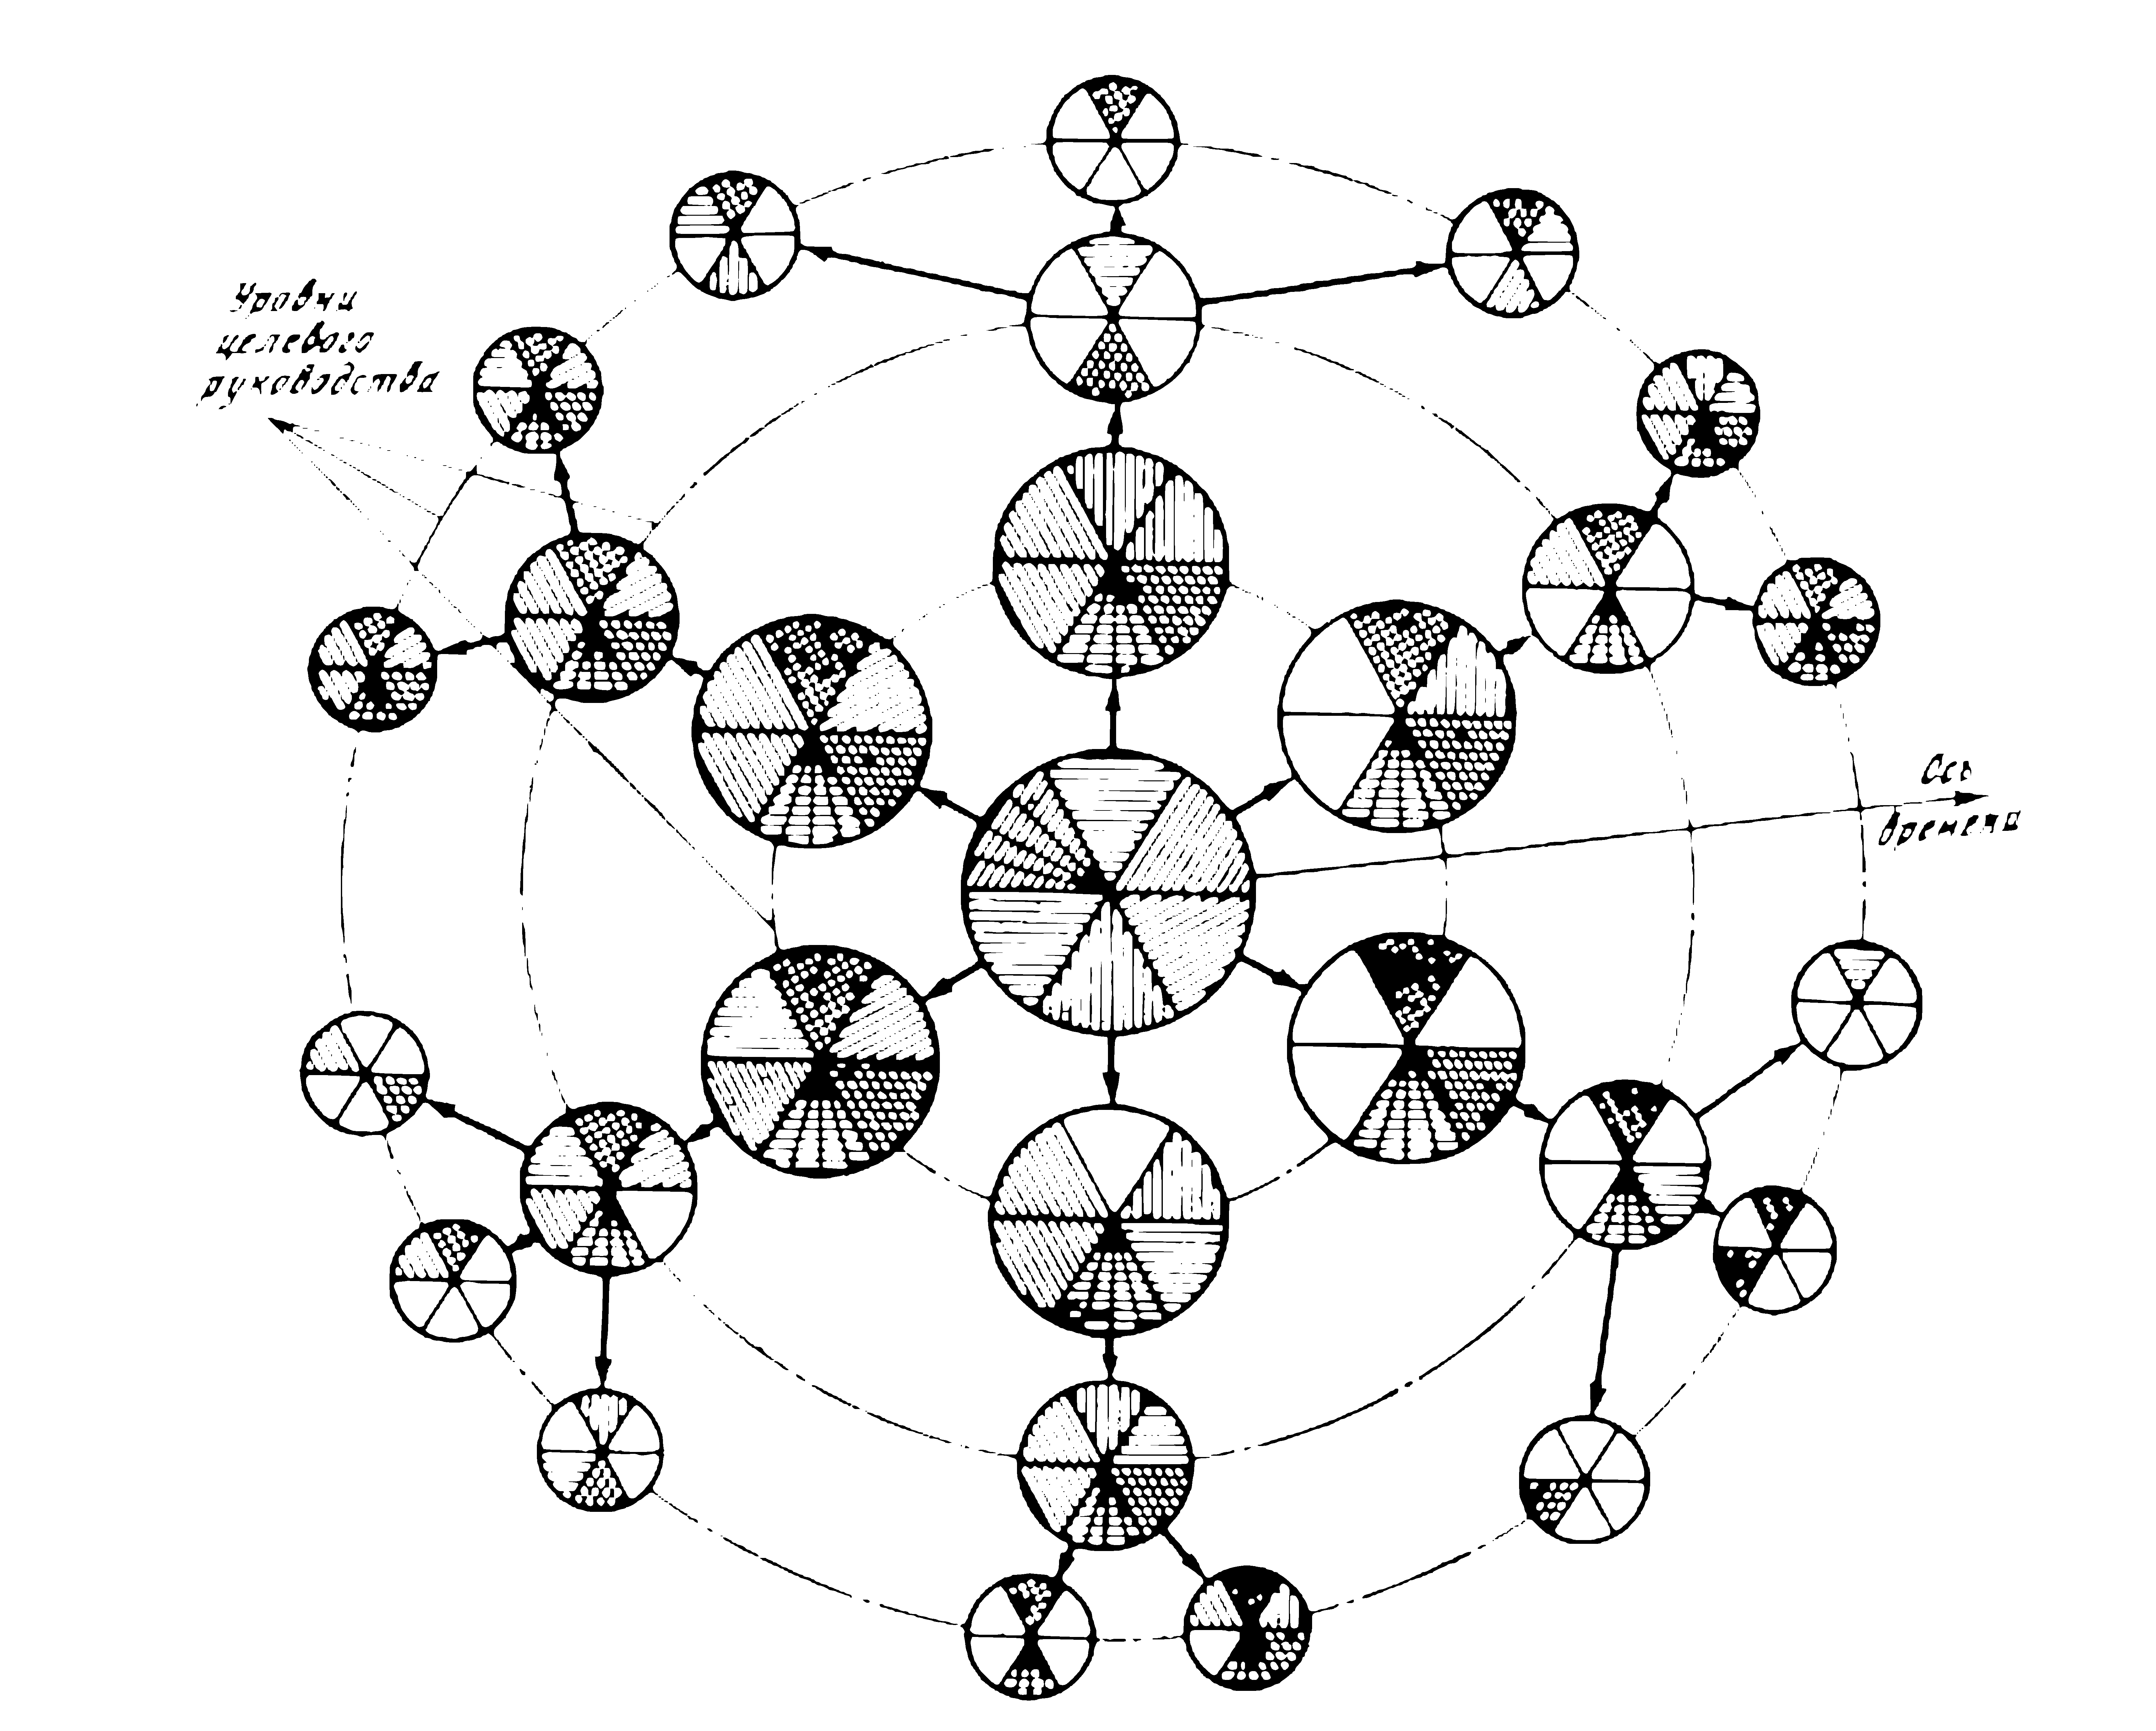
\includegraphics[width=\linewidth]{assets/figure-P4-vector.pdf}
\caption{Рис. П.4. Векторная трассировка карты хода разработки; S-02, с. 129; перенос из S-01, с. 114, рис. 14.}
\end{figure}
\clearpage
\begin{figure}[p]\centering
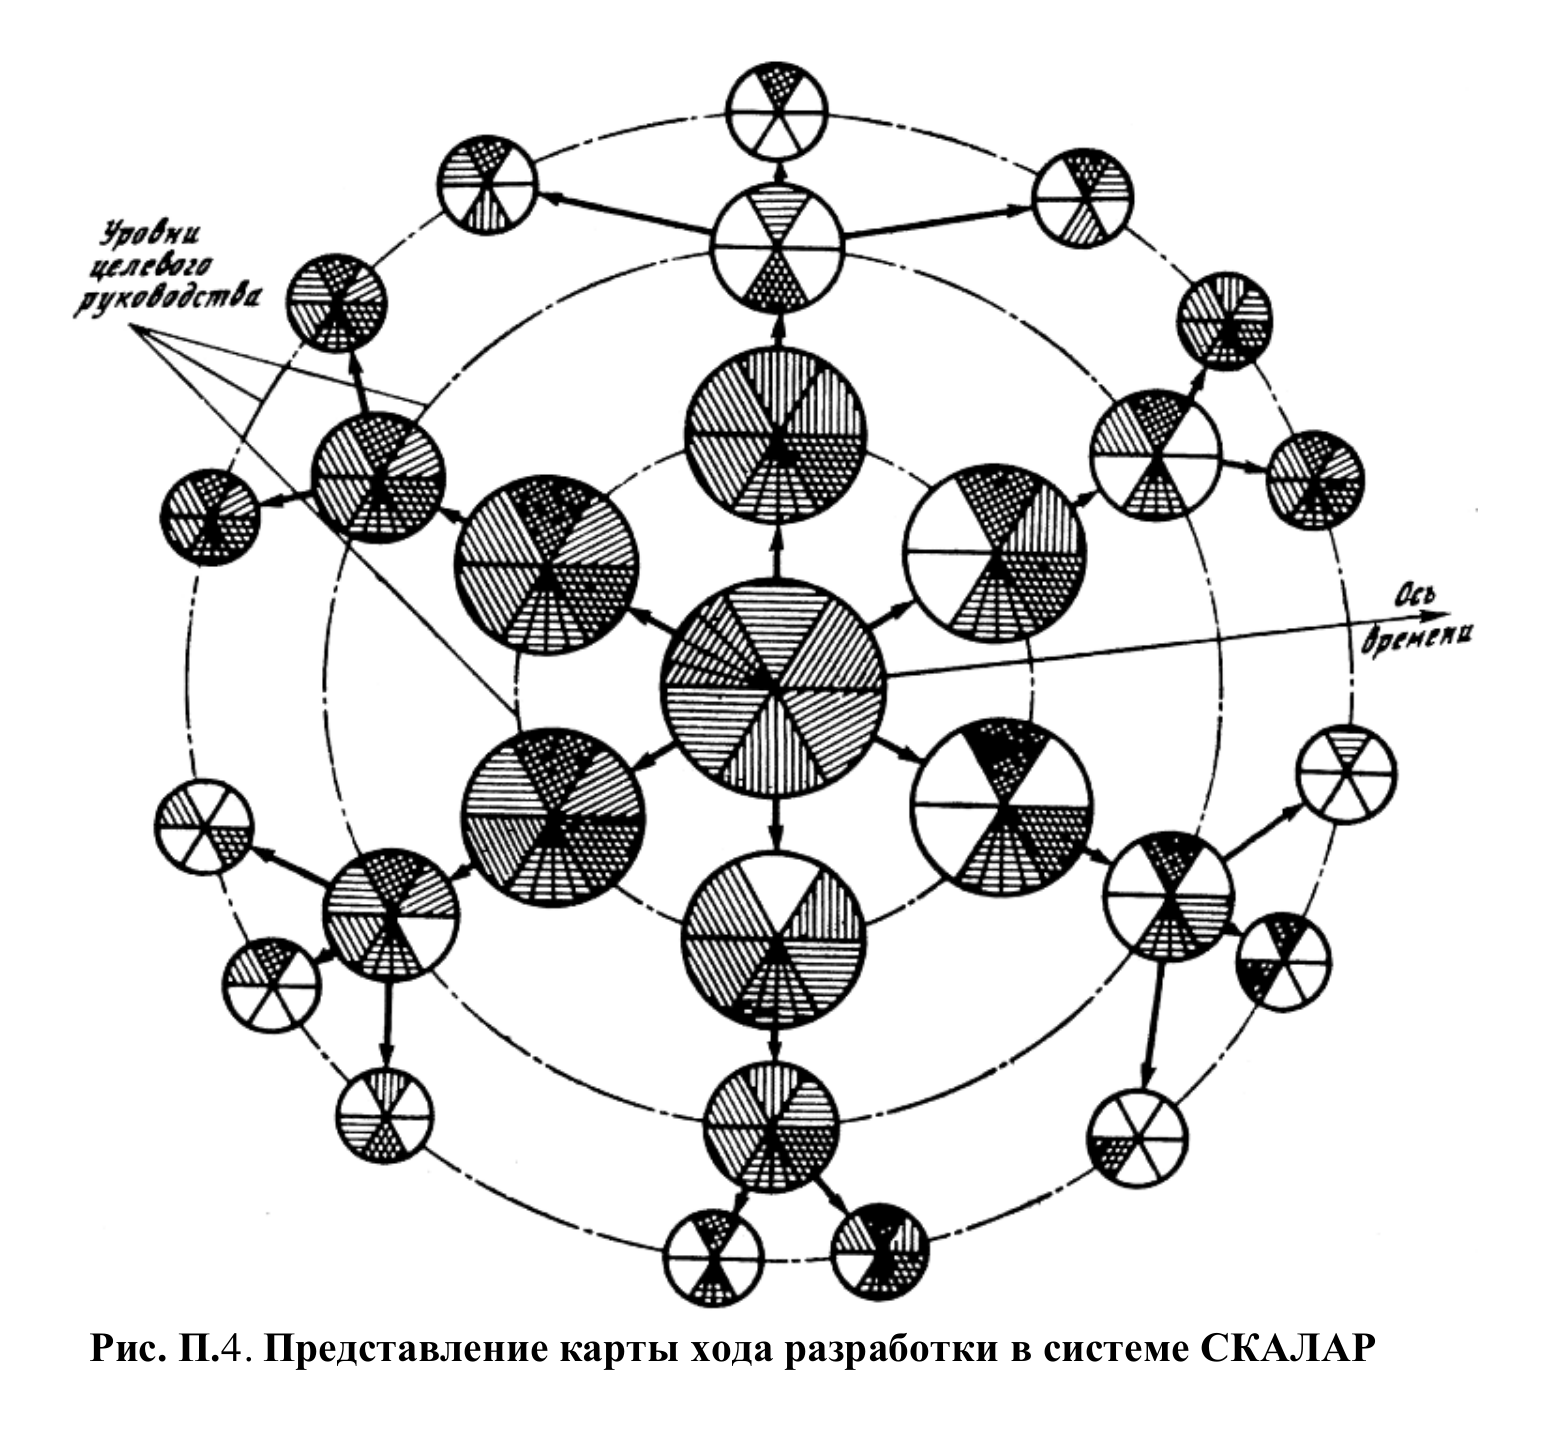
\includegraphics[width=0.96\linewidth]{assets/source-P4.png}
\caption{Контрольное факсимиле рисунка П.4 по S-02, с. 129.}
\end{figure}

\clearpage
\section{Формы таблиц П.1--П.9}\label{sec:forms}

Пустые клетки оставлены пустыми, как в источнике. Шапки и объединения ячеек набраны заново; нумерация столбцов сохранена. В П.9 верхняя таблица и нижняя матрица соприкасаются в ступенчатом углу, как на исходной странице; подпись остаётся слева от матрицы.

\subsection{Таблица П.1. Лист согласования}
\formsource{116}{178}
\formmetadata{Шифр организации\\Шифр подразделения\\Шифр ОИР\\Тел.}
\footnotesize
\setlength{\tabcolsep}{1.5pt}
\begin{tabularx}{\dimexpr\linewidth-15pt\relax}{|c|X|X|c|X|X|}\hline
\multicolumn{6}{|c|}{РЕЗУЛЬТАТЫ}\\\hline
\multirow{2}{*}{№ п/п}&\multicolumn{2}{c|}{принимаемые}&\multirow{2}{*}{№ п/п}&\multicolumn{2}{c|}{выдаваемые}\\\cline{2-3}\cline{5-6}
&Шифр поставщика&Краткое описание&&Шифр получателя&Краткое описание\\\hline
\blankrow&&&&&\\\hline
\end{tabularx}

\clearpage
\subsection{Таблица П.2. Запрос на сетевую документацию}
\formsource{117}{179}
\formmetadata{Шифр организации\\Шифр подразделения\\Шифр ОИР\\Тел.}
\begin{tabularx}{\dimexpr\linewidth-15pt\relax}{|c|X|X|c|X|X|}\hline
\multicolumn{6}{|c|}{РЕЗУЛЬТАТЫ}\\\hline
\multirow{2}{*}{№ п/п}&\multicolumn{2}{c|}{принимаемые}&\multirow{2}{*}{№ п/п}&\multicolumn{2}{c|}{выдаваемые}\\\cline{2-3}\cline{5-6}
&Шифр поставщика&Краткое описание&&Шифр получателя&Краткое описание\\\hline
\blankrow&&&&&\\\hline
\end{tabularx}

\clearpage
\subsection{Таблица П.3. Исходные данные по работам}
\formsource{118}{180}
\formmetadata{Шифр организации\\Шифр подразделения\\Шифр ОИР\\Тел.}
\setlength{\tabcolsep}{1.5pt}
\begin{tabularx}{\dimexpr\linewidth-15pt\relax}{|c|X|X|c|c|X|X|}\hline
№ п/п&Шифр поставщика (получателя)&Код следования результата&\multicolumn{2}{c|}{Шифры событий}&Краткое описание работы&Оценка длительности\\\cline{4-5}
&&&начало&конец&&\\\hline
\blankrow&&&&&&\\\hline
\end{tabularx}

\clearpage
\begin{landscape}
\subsection{Таблица П.4. Состояние работ по цели}
\formsource{121}{183}
\scriptsize
\setlength{\tabcolsep}{2pt}
\formmetadata{Шифр организации\\Шифр подразделения\\Шифр ЦР\\Тел.}
\resizebox{0.97\linewidth}{!}{%
\begin{tabular}{|V|V|V|V|V|V|V|V|V|V|V|V|}\hline
\vheadland{№ п/п}&\vheadland{Шифр поставщика (получателя)}&\vheadland{Код следования результата}&\multicolumn{2}{c|}{Шифр событий}&\vheadland{Краткое описание работ}&\multicolumn{3}{c|}{Оценка длительности}&\vheadland{Дата по графику}&\vheadland{Резерв (полный) окончания работы}&\vheadland{Примечание}\\\cline{4-5}
&&&\vheadland{начало}&\vheadland{конец}&&&&& & & \\[-1.3em]
1&2&3&4&5&6&7&8&9&10&11&12\\\hline
\blankrow&&&&&&&&&&&\\\hline
\end{tabular}}

\medskip
\clearpage
\subsection{Таблица П.5. Состояние работ по подразделению}
\formsource{121}{183}
\formmetadata{Шифр организации\\Шифр подразделения\\Шифр РП\\Тел.}
\resizebox{0.97\linewidth}{!}{%
\begin{tabular}{|V|V|V|V|V|V|V|V|V|V|V|V|}\hline
\vheadland{№ п/п}&\vheadland{Шифр поставщика (получателя)}&\vheadland{Код следования результата}&\multicolumn{2}{c|}{Шифр событий}&\vheadland{Краткое описание работ}&\multicolumn{3}{c|}{Оценка длительности}&\vheadland{Дата по графику}&\vheadland{Резерв (полный) окончания работы}&\vheadland{Примечание}\\\cline{4-5}
&&&\vheadland{начало}&\vheadland{конец}&&&&&&&\\[-1.3em]
1&2&3&4&5&6&7&8&9&10&11&12\\\hline
\blankrow&&&&&&&&&&&\\\hline
\end{tabular}}
\par\smallskip\noindent\parbox{\linewidth}{\footnotesize В источнике таблица П.5 напечатана с сокращением «СРЦ». В окружающем тексте она названа состоянием работ по подразделению и сокращена как «СРП»; ошибка или вариант источника не исправлены молча.}

\clearpage
\subsection{Таблица П.6. Запрос данных о работах}
\formsource{122}{184}
\scriptsize
\setlength{\tabcolsep}{2pt}
\formmetadata{Шифр организации\\Шифр подразделения\\Шифр ОИР\\Тел.}
\resizebox{0.97\linewidth}{!}{%
\begin{tabular}{|V|V|V|V|V|V|V|V|V|V|V|V|V|V|V|}\hline
\multicolumn{9}{|c|}{Из ЗДР}&&&&\multicolumn{2}{c|}{Фактическая дата}&\multirow{3}{*}{\vhead{Примечание}}\\\cline{1-9}\cline{13-14}
\vheadland{№ п/п}&\vheadland{Шифр поставщика (получателя)}&\vheadland{Код следования результата}&\multicolumn{2}{c|}{Шифр событий}&\vheadland{Краткое описание работ}&\multicolumn{3}{c|}{Оценка длительности}&\vheadland{Завершение работы (дата по графику)}&\vheadland{Резерв (полный) окончания работы}&\vheadland{Код изменений}&\vheadland{начало}&\vheadland{конец}&\\\cline{4-5}
&&&\vheadland{начало}&\vheadland{конец}&&&&&&&&&&\\[-1.4em]
1&2&3&4&5&6&7&8&9&10&11&12&13&14&15\\\hline
\blankrow&&&&&&&&&&&&&&\\\hline
\end{tabular}}

\clearpage
\subsection{Таблица П.7. Запрос на изменение сети}
\formsource{123}{185}
\setlength{\tabcolsep}{2pt}
\formmetadata{Шифр организации\\Шифр подразделения\\Шифр ОИР\\Тел.}
\resizebox{0.97\linewidth}{!}{%
\begin{tabular}{|V|V|V|V|V|V|V|V|V|V|V|V|}\hline
\multicolumn{11}{|c|}{Что было в ЗДР}&\multirow{3}{*}{\rotatebox[origin=c]{90}{\parbox{5cm}{\centering\scriptsize Что желательно иметь}}}\\\cline{1-11}
\vheadland{№ п/п}&\vheadland{Шифр поставщика (получателя)}&\vheadland{Код следования результата}&\multicolumn{2}{c|}{Шифр событий}&\vheadland{Краткое описание работ}&\multicolumn{3}{c|}{Оценка длительности}&\vheadland{Дата по графику}&\vheadland{Резерв (полный) окончания работы}&\\\cline{4-5}
&&&\vheadland{начало}&\vheadland{конец}&&&&&&&\\[-1.4em]
1&2&3&4&5&6&7&8&9&10&11&12\\\hline
\blankrow&&&&&&&&&&&\\\hline
\end{tabular}}

\clearpage
\subsection{Таблица П.8. Изменение рабочей сети}
\formsource{124}{186}
\setlength{\tabcolsep}{2pt}
\formmetadata{Шифр организации\\Шифр подразделения\\Шифр ОИР\\Тел.}
\resizebox{0.97\linewidth}{!}{%
\begin{tabular}{|V|V|V|V|V|V|V|V|V|V|V|V|V|V|V|}\hline
\multicolumn{4}{|c|}{Что было в ИДР}&&\multicolumn{8}{c|}{Что должно быть в ИДР}&\multicolumn{2}{c|}{Согласовано}\\\cline{1-4}\cline{6-13}\cline{14-15}
\vheadland{Шифр поставщика (получателя)}&\vheadland{Код следования результата}&\multicolumn{2}{c|}{Шифр событий}&\multirow{2}{*}{\vheadland{Код изменения}}&\vheadland{Шифр поставщика (получателя)}&\vheadland{Код следования результата}&\multicolumn{2}{c|}{Шифр событий}&\vheadland{Краткое описание работы}&\multicolumn{3}{c|}{Оценка длительности}&\vheadland{Шифр}&\vheadland{Подпись}\\\cline{3-4}\cline{8-9}
& &\vheadland{начало}&\vheadland{конец}&&&&\vheadland{начало}&\vheadland{конец}&&&&&&\\[-1.4em]
1&2&3&4&5&6&7&8&9&10&11&12&13&14&15\\\hline
\blankrow&&&&&&&&&&&&&&\\\hline
\end{tabular}}
\end{landscape}

\subsection{Таблица П.9. Отчёт о ходе работ}
\formsource{127}{188}
\noindent\resizebox{\linewidth}{!}{%
\begin{tikzpicture}[baseline=(upper.north)]
\node[anchor=north west,inner sep=0pt,outer sep=0pt] (metadata) at (0,0) {\footnotesize
\begin{tabular}{@{}p{7.27cm}@{}}
По теме: \rule{1.2cm}{0.35pt}\hfill Дата засечки: \rule{1cm}{0.35pt}\\
Шифр организации: \rule{2.3cm}{0.35pt}\\
Целевой руководитель: \rule{2cm}{0.35pt}\\
\end{tabular}};
\node[anchor=north west,inner sep=0pt,outer sep=0pt] (upper) at (metadata.south west) {\footnotesize
\begin{tabular}{|p{3.8cm}|p{1.1cm}|p{1.1cm}|}\hline
\rule{0pt}{4.4cm}&\vhead{Директивный}&\vhead{Ожидаемый}\\\hline
Срок окончания&&\\\hline
Объём финансирования&&\\\hline
\end{tabular}};
\node[anchor=north west,inner sep=0pt,outer sep=0pt] at (upper.south east) {\scriptsize
\begin{tabular}{|>{\centering\arraybackslash}p{0.5cm}|p{1.8cm}|>{\centering\arraybackslash}p{1.3cm}|>{\centering\arraybackslash}p{1.3cm}|>{\centering\arraybackslash}p{1.2cm}|p{2.1cm}|}\hline
\multicolumn{2}{|c|}{}&\vhead{Должно быть}&\vhead{Фактически}&\multicolumn{2}{c|}{Требует решений}\\\cline{5-6}
\rule{0pt}{4.3cm}\vhead{№}& & & &\vhead{Сколько}&\vhead{№ контрольных карточек}\\\hline
1&Кто&&&&\\\hline
2&Что&&&&\\\hline
3&Когда&&&&\\\hline
4&Где&&&&\\\hline
5&Сколько&&&&\\\hline
6&Как&&&&\\\hline
\multicolumn{2}{|l|}{РЕАЛИЗАЦИЯ}&&&&\\\hline
\end{tabular}};
\node[anchor=north west,inner sep=0pt,outer sep=0pt] at (upper.south west) {\begin{minipage}[t]{6.9cm}\vspace*{8.8cm}Подпись: \rule{3cm}{0.35pt}.\end{minipage}};
\end{tikzpicture}}

\section{Контрольные факсимиле исходных рисунков}\label{sec:facsimiles}

Факсимиле нужны для проверки линий, штриховок, разветвлений и чтения мелких надписей. Для П.3--П.4 источник тома 5 сообщает, что составители перенесли рисунки из книги 1996 года, страница 114.

\begin{figure}[p]\centering
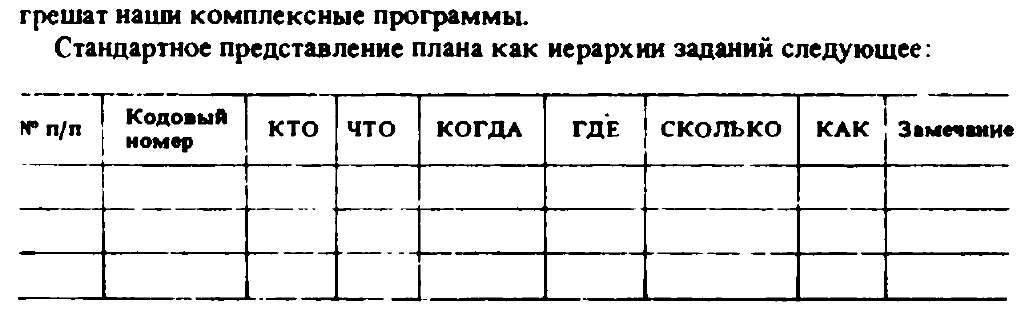
\includegraphics[width=0.96\linewidth]{assets/source-book96-plan-row.png}
\caption{Фрагмент страницы 113 книги 1996 года: стандартная строка плана СКАЛАР.}
\end{figure}
\begin{figure}[p]\centering
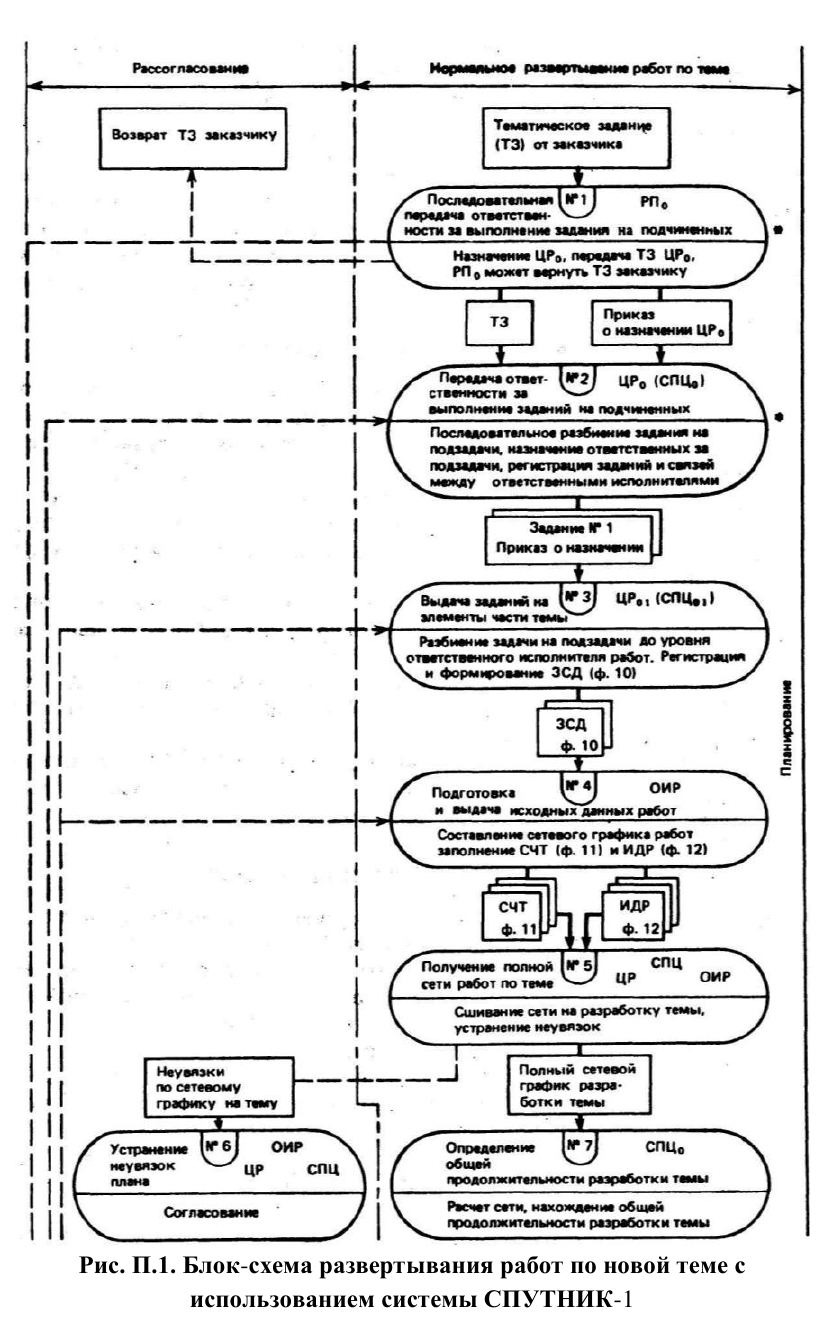
\includegraphics[width=0.48\linewidth]{assets/source-P1a.png}\hfill
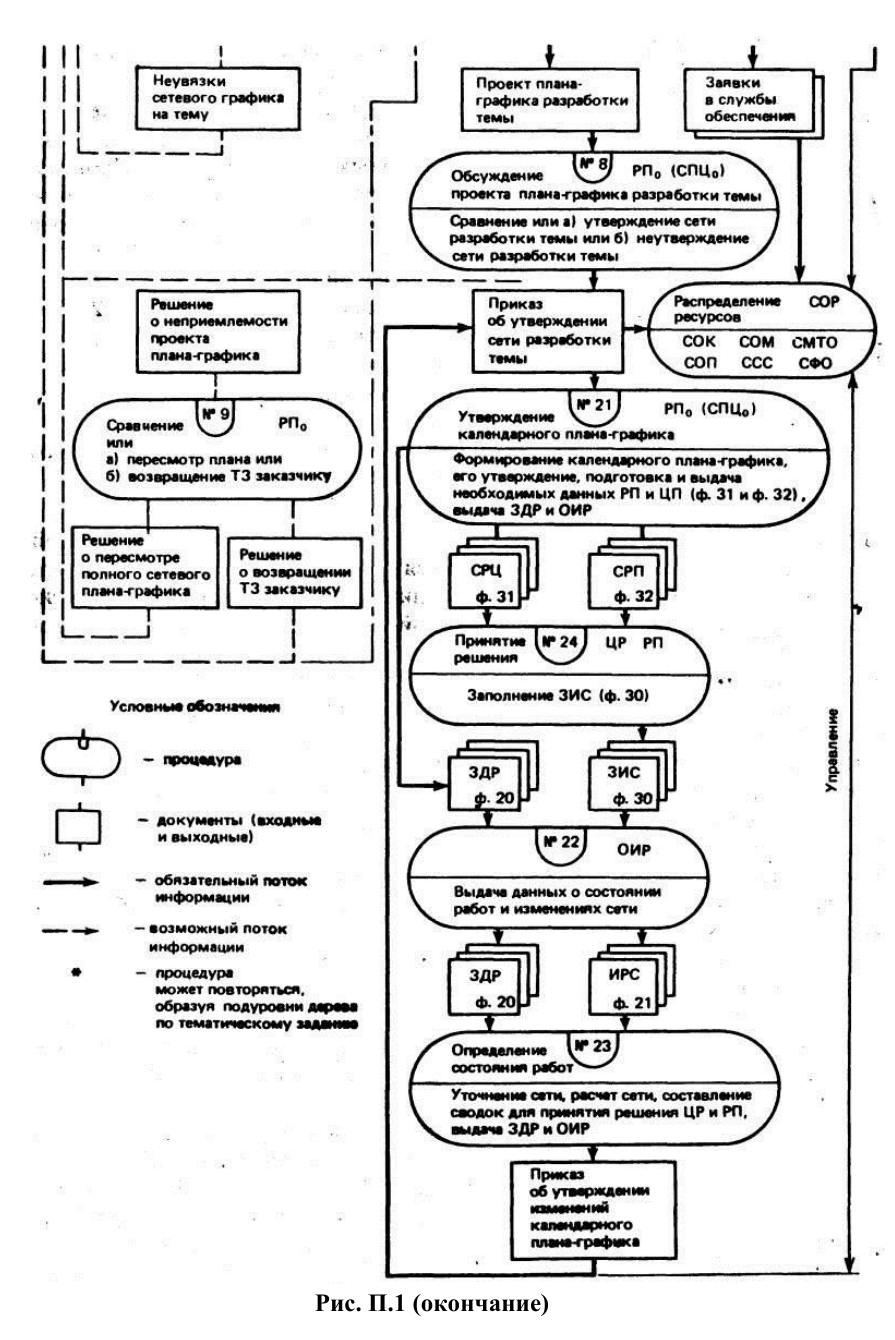
\includegraphics[width=0.48\linewidth]{assets/source-P1b.png}
\caption{Рис. П.1, источник: S-02, с. 113--114.}
\end{figure}
\begin{figure}[p]\centering
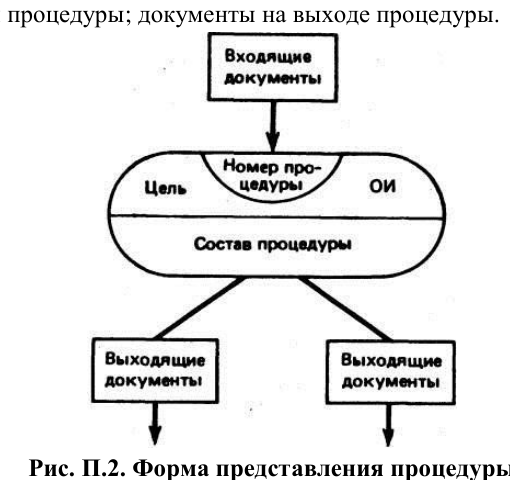
\includegraphics[width=0.43\linewidth]{assets/source-P2.png}\hfill
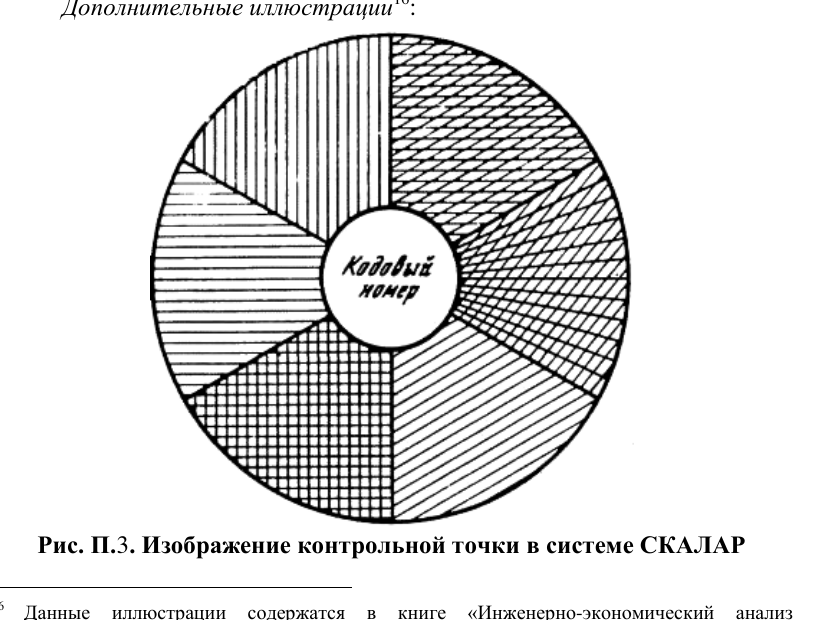
\includegraphics[width=0.54\linewidth]{assets/source-P3.png}
\caption{Рис. П.2 и П.3, источник: S-02, с. 115 и 128.}
\end{figure}

\clearpage
\section{Полные факсимиле страниц исходных PDF}

Факсимиле сохраняют исходные таблицы, рисунки, подписи, расположение текста и ошибки печати. Текстовые слои и восстановленные формы выше остаются поисковой и наборной версиями; сканы ниже дают полный постраничный контроль.

\subsection{Том 5, страницы 11--129}

\includepdf[pages=11-129,fitpaper=true,pagecommand={}]{../sources/originals/Kuznetsov-Nauka-Razvitiya-Zhizni-Vol5-2021.pdf}

\subsection{Книга 1996 года, страницы 111--118}

\includepdf[pages=111-118,fitpaper=true,pagecommand={}]{../sources/originals/Obraztsova-Kuznetsov-Pshenichnikov-Transport-Systems-1996.pdf}

\section*{Источники}
\addcontentsline{toc}{section}{Источники}
\begin{enumerate}
\item Образцова Р. И., Кузнецов П. Г., Пшеничников С. Б. \textit{Инженерно-экономический анализ транспортных систем: Методология проектирования автоматизированной системы управления}. 2-е стереотипное изд. М.: Радио и связь, 1996. С. 111--118, 173--189; рис. 13--14 на с. 114.
\item Кузнецов П. Г. \textit{Наука развития Жизни: сборник трудов. Том 5. Введение в сетевое планирование. Работы разных лет}. М.—Дубна, 2021. С. 11--129. Редакторы-составители Е. Ф. Шамаева, Е. Б. Попов. Включённые тексты и редакторские границы перечислены в реестре первичных материалов.
\end{enumerate}

\end{document}
